\chap{3D旋转变换}
\section{介绍}
在本章中,我们回顾了在计算机图形软件中使用的三维欧拉旋转变换。特别地,我们确定了他们的阿喀琉斯之踵——万向节锁——以及能够围绕任意轴旋转的需求。为此,我们将开发一个实现这种旋转的矩阵变换,并在下一章中使用四元数开发一个类似的变换。

\section{3D旋转变换}
旋转点和参考系的传统技术是基于欧拉旋转,以瑞士数学家Leonhard Euler的名字命名。他们提供了三种轮换的方法。第一种是绕三个笛卡尔轴之一旋转。第二个组合了任意两个围绕不同轴的旋转,第三个组合了任意三个旋转。

最初,这种方法听起来很吸引人——在许多情况下效果很好,然而,这种技术存在一些问题。第一个问题是,当两个或多个旋转结合在一起时,很难可视化和预测最终的旋转将如何表现。第二点是,绕一个特定的轴旋转是很复杂的,第三点是,在某些条件下,人们失去了对物体的一个旋转轴的访问。最后一个问题被称为万向节锁。为了理解这些问题,我们将构建一个受万向节锁定影响的三维旋转变换。

\section{绕笛卡尔轴旋转}
一个点在平面上绕原点旋转的变换由
$$
\mathbf{R}_{\beta}=\left[\begin{array}{cc}
\cos \beta & -\sin \beta \\
\sin \beta & \cos \beta
\end{array}\right] .
$$

这可以通过添加第三个坐标推广到围绕笛卡尔轴的三维旋转。例如,要绕$z$-轴旋转,我们添加一个$z$-坐标,如下所示:
$$
\mathbf{R}_{\beta, z}=\left[\begin{array}{ccc}
\cos \beta & -\sin \beta & 0 \\
\sin \beta & \cos \beta & 0 \\
0 & 0 & 1
\end{array}\right]
$$

\begin{figure}[h!]
    \centering
    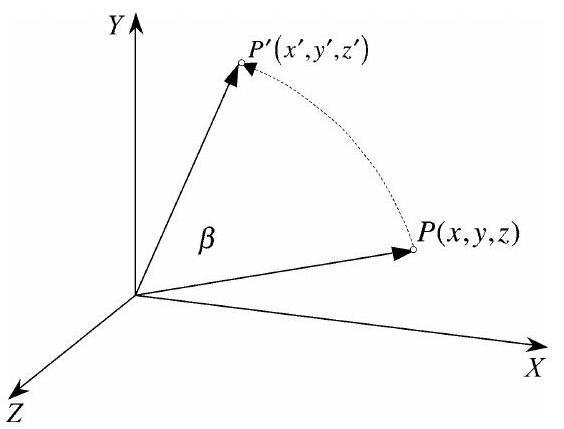
\includegraphics[max width=0.5\textwidth]{2023_01_16_a848224efad29cd66460g-089}
    \caption[short]{点 $P$ 围绕 $z$ 轴旋转}
\end{figure}

如图6.1所示。要围绕$x$-轴旋转一个点,$x$-坐标保持不变,而$y$ -和$z$-坐标根据$2 \mathrm{D}$旋转变换进行更改:
$$
\mathbf{R}_{\beta, x}=\left[\begin{array}{ccc}
1 & 0 & 0 \\
0 & \cos \beta & -\sin \beta \\
0 & \sin \beta & \cos \beta
\end{array}\right] .
$$

最后,为了绕$y$-轴旋转,$y$-坐标保持不变,而$x$和$z$-坐标改变:
$$
\mathbf{R}_{\beta, y}=\left[\begin{array}{ccc}
\cos \beta & 0 & \sin \beta \\
0 & 1 & 0 \\
-\sin \beta & 0 & \cos \beta
\end{array}\right] .
$$

\section{绕偏移轴旋转}
要绕与笛卡尔轴之一平行的轴旋转,通常采用齐次坐标并平移要旋转的点,这样它可以绕原点旋转,然后平移回来一个相等且相反的量。假定读者熟悉这种策略。但是,为了完整起见,我们将构造一个变换,使一个点围绕一个与$z$-轴平行的轴旋转,并与点$\left(t_{x}, t_{y}, 0\right)$相交,如图6.2所示:
$$
\left[\begin{array}{c}
x^{\prime} \\
y^{\prime} \\
z^{\prime} \\
1
\end{array}\right]=\mathbf{T}_{t_{x}, t_{y}, 0} \mathbf{R}_{\beta, z} \mathbf{T}_{-t_{x},-t_{y}, 0}\left[\begin{array}{c}
x \\
y \\
z \\
1
\end{array}\right]
$$

\begin{figure}
    \centering
    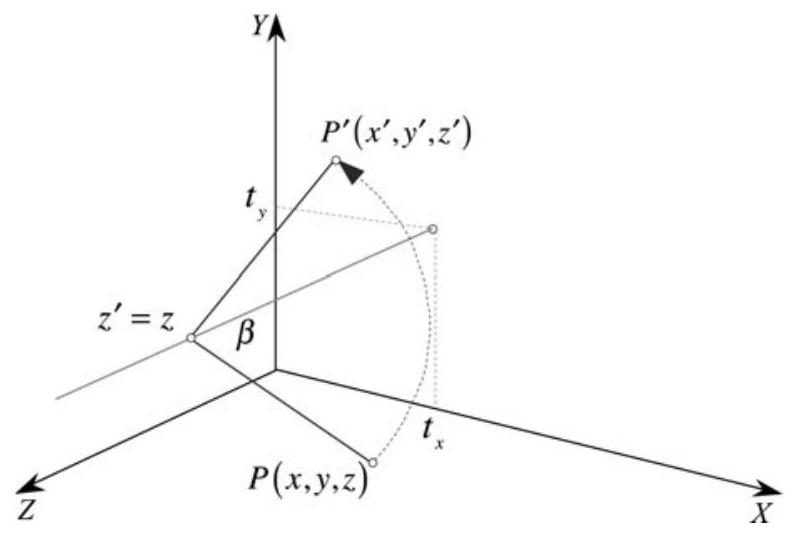
\includegraphics[max width=0.6\textwidth]{2023_01_16_a848224efad29cd66460g-090}
    \caption[short]{绕平行于$z$-轴的轴旋转一点}
\end{figure}

其中
$$
\begin{aligned}
& \mathbf{T}_{-t_{x},-t_{y}, 0} && \text { 创建临时原点 } \\
& \mathbf{R}_{\beta, z} && \beta \text { 围绕临时的 } z \text {轴旋转 } \\
& \mathbf{T}_{t_{x}, t_{y}, 0} && \text { 回到原来的坐标系中的位置 }
\end{aligned}
$$

矩阵变换是
$$
\mathbf{R}_{\beta, z,\left(t_{x}, t_{y}, 0\right)}=\left[\begin{array}{cccc}
\cos \beta & -\sin \beta & 0 & t_{x}(1-\cos \beta)+t_{y} \sin \beta \\
\sin \beta & \cos \beta & 0 & t_{y}(1-\cos \beta)-t_{x} \sin \beta \\
0 & 0 & 1 & 0 \\
0 & 0 & 0 & 1
\end{array}\right]
$$

围绕平行于$x$-轴和平行于$y$-轴的偏移轴旋转的矩阵为:
$$
\begin{aligned}
\mathbf{R}_{\beta, x,\left(0, t_{y}, t_{z}\right)} & =\left[\begin{array}{cccc}
1 & 0 & 0 & 0 \\
0 & \cos \beta & -\sin \beta & t_{y}(1-\cos \beta)+t_{z} \sin \beta \\
0 & \sin \beta & \cos \beta & t_{z}(1-\cos \beta)-t_{y} \sin \beta \\
0 & 0 & 0 & 1
\end{array}\right] \\
\mathbf{R}_{\beta, y,\left(t_{x}, 0, t_{z}\right)} & =\left[\begin{array}{cccc}
\cos \beta & 0 & \sin \beta & t_{x}(1-\cos \beta)-t_{z} \sin \beta \\
0 & 1 & 0 & 0 \\
-\sin \beta & 0 & \cos \beta & t_{z}(1-\cos \beta)+t_{x} \sin \beta \\
0 & 0 & 0 & 1
\end{array}\right] .
\end{aligned}
$$

\section{复合旋转}
撇开围绕单轴和偏移轴旋转的变换不谈,我们有三个围绕笛卡尔轴旋转的变换:$\mathbf{R}_{\alpha, x}, \mathbf{R}_{\beta, y}$和$\mathbf{R}_{\gamma, z}$,它们可以组合成双变换族和三重变换族。如上所述,这种旋转称为欧拉旋转,假定读者熟悉其结构。三重变换族是:
$$
\begin{array}{llll}
\mathbf{R}_{\gamma, x} \mathbf{R}_{\beta, y} \mathbf{R}_{\alpha, x} & \mathbf{R}_{\gamma, x} \mathbf{R}_{\beta, y} \mathbf{R}_{\alpha, z} & \mathbf{R}_{\gamma, x} \mathbf{R}_{\beta, z} \mathbf{R}_{\alpha, x} & \mathbf{R}_{\gamma, x} \mathbf{R}_{\beta, z} \mathbf{R}_{\alpha, y} \\
\mathbf{R}_{\gamma, y} \mathbf{R}_{\beta, x} \mathbf{R}_{\alpha, y} & \mathbf{R}_{\gamma, y} \mathbf{R}_{\beta, x} \mathbf{R}_{\alpha, z} & \mathbf{R}_{\gamma, y} \mathbf{R}_{\beta, z} \mathbf{R}_{\alpha, x} & \mathbf{R}_{\gamma, y} \mathbf{R}_{\beta, z} \mathbf{R}_{\alpha, y} \\
\mathbf{R}_{\gamma, z} \mathbf{R}_{\beta, x} \mathbf{R}_{\alpha, y} & \mathbf{R}_{\gamma, z} \mathbf{R}_{\beta, x} \mathbf{R}_{\alpha, z} & \mathbf{R}_{\gamma, z} \mathbf{R}_{\beta, y} \mathbf{R}_{\alpha, x} & \mathbf{R}_{\gamma, z} \mathbf{R}_{\beta, y} \mathbf{R}_{\alpha, z} .
\end{array}
$$

为了说明万向节锁的问题,我们将使用一个立方体,其顶点编号为0到7,如图6.3所示。
\begin{figure}[h!]
    \centering
    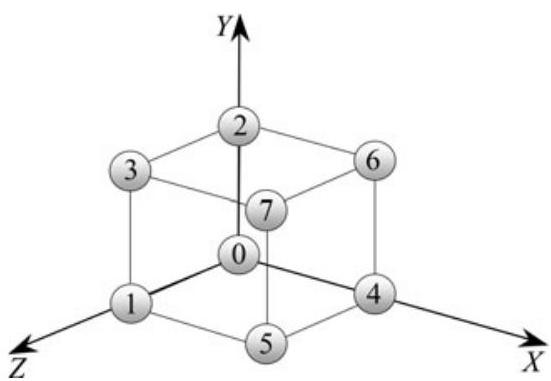
\includegraphics[max width=0.5\textwidth]{2023_01_16_a848224efad29cd66460g-091}
    \caption[short]{位于原点的单位立方体}
\end{figure}
\begin{figure}[h!]
    \centering
    \subfigure[]{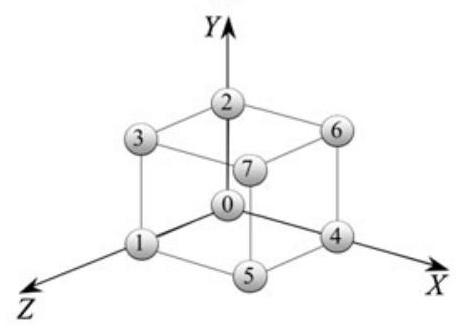
\includegraphics[max width=0.4\textwidth]{2023_01_16_a848224efad29cd66460g-091(1)}}
    \subfigure[]{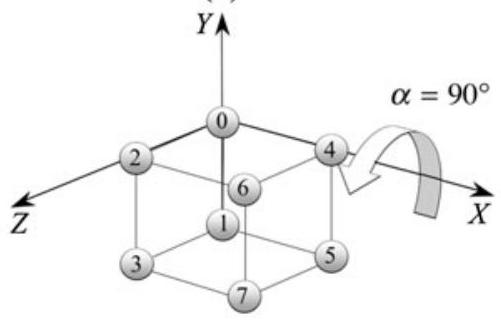
\includegraphics[max width=0.4\textwidth]{2023_01_16_a848224efad29cd66460g-091(3)}}\\
    \subfigure[]{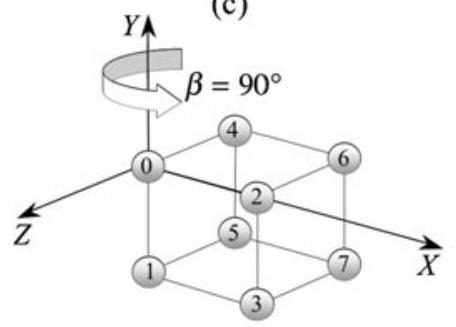
\includegraphics[max width=0.4\textwidth]{2023_01_16_a848224efad29cd66460g-091(2)}}
    \subfigure[]{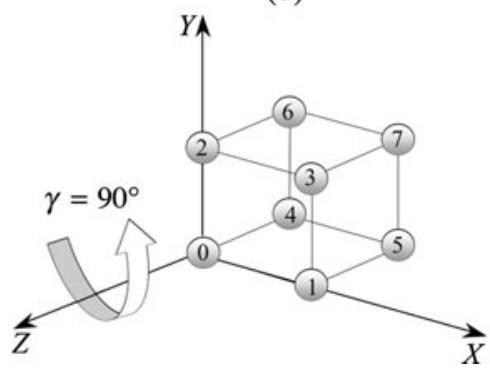
\includegraphics[max width=0.4\textwidth]{2023_01_16_a848224efad29cd66460g-091(4)}}
    \caption[short]{单位立方体在三次旋转之前和期间的四个视图}
\end{figure}

我们可以通过在任意序列中放置$\mathbf{R}_{\alpha, x}, \mathbf{R}_{\beta, y}$和$\mathbf{R}_{\gamma, z}$来创建复合旋转变换——甚至可以重复其中一个序列两次,只要它们被不同的变换隔开。作为后者的一个例子,我们可以使用序列$\mathbf{R}_{\alpha, z} \mathbf{R}_{\beta, y} \mathbf{R}_{\gamma, z}$,其中我们围绕$z$-轴旋转两次。然而,为了说明万向节锁,让我们选择序列$\mathbf{R}_{\gamma, z} \mathbf{R}_{\beta, y} \mathbf{R}_{\alpha, x}$,并使$\alpha=\beta=\gamma=90^{\circ}$,这相当于围绕固定的$x$-轴旋转一个点$90^{\circ}$,然后围绕固定的$y$-轴旋转$90^{\circ}$,然后围绕固定的$z$-轴旋转$90^{\circ}$。该旋转序列如图6.4所示。

\begin{figure}[h!]
    \centering
    \subfigure[]{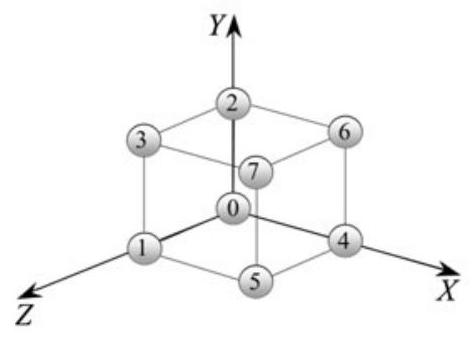
\includegraphics[max width=0.4\textwidth]{2023_01_16_a848224efad29cd66460g-092}}
    \subfigure[]{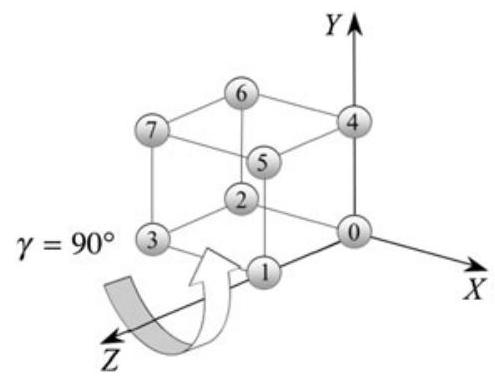
\includegraphics[max width=0.4\textwidth]{2023_01_16_a848224efad29cd66460g-092(2)}}\\
    \subfigure[]{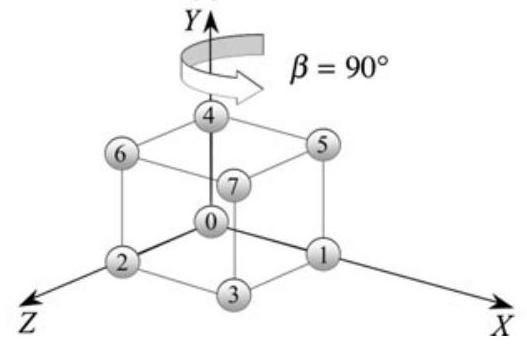
\includegraphics[max width=0.4\textwidth]{2023_01_16_a848224efad29cd66460g-092(1)}}
    \subfigure[]{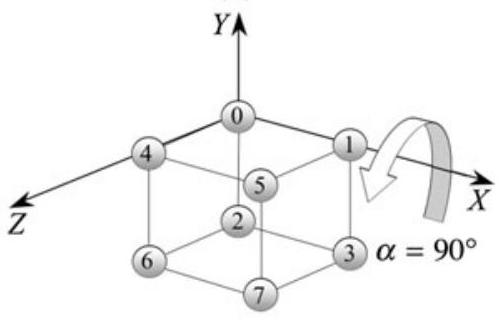
\includegraphics[max width=0.4\textwidth]{2023_01_16_a848224efad29cd66460g-092(3)}}
    \caption[short]{使用旋转序列$\mathbf{R}_{\alpha, x} \mathbf{R}_{\beta, y} \mathbf{R}_{\gamma, z}$的单位立方体的四个视图}
\end{figure}


Figure $6.4$ (a) shows the starting position of the cube; (b) shows its position after a $90^{\circ}$ rotation about the $x$-axis; (c) shows its position after a further rotation of $90^{\circ}$ about the $y$-axis; and (d) the cube's resting position after a rotation of $90^{\circ}$ about the z-axis.

However, in spite of employing three rotations about different axes, the cube has effectively only been rotated $90^{\circ}$ about the $y$-axis! The cube has been rotated twice about the axis passing through vertices 0 and 4 and once about the axis passing through vertices 0 and 1 , but the axis passing through vertices 0 and 2 has been ignored. This is known as gimbal lock, and arises through an unfortunate rotation sequence combination and angles.

Reversing the composite rotation to $\mathbf{R}_{\alpha, x} \mathbf{R}_{\beta, y} \mathbf{R}_{\gamma, z}$ does not improve matters. This composite transform is equivalent to rotating a point $90^{\circ}$ about the fixed zaxis, followed by a rotation of $90^{\circ}$ about the fixed $y$-axis, followed by a rotation of $90^{\circ}$ about the fixed $x$-axis. This rotation sequence is illustrated in Fig. 6.5.

Inspection of Fig. $6.5$ (d) shows that the unit cube has been rotated $180^{\circ}$ about the vector $\left[\begin{array}{lll}1 & 0 & 1\end{array}\right]^{\mathrm{T}}$, i.e. an axis intersecting vertices 0 and 5. This time, the cube is rotated twice about an axis intersecting vertices 0 and 1 , once about an axis intersecting vertices 0 and 4 , and once again, the axis intersecting vertices 0 and 2 has 

\begin{figure}[h!]
    \centering
    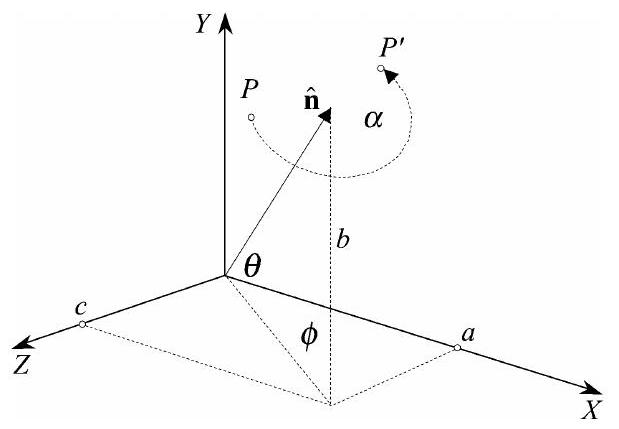
\includegraphics[max width=0.5\textwidth]{2023_01_16_a848224efad29cd66460g-093}
    \caption[short]{绕任意轴旋转的几何图形}
\end{figure}

been ignored. It is not difficult to see why Euler rotations cause so many problems. So let's continue and see how we can rotate about an arbitrary axis.

\section{绕任意轴旋转}
There is nothing fundamentally wrong with individual Euler transforms-it is the way they are combined to effect a rotation that is flawed. Ideally, we require a rotation transform that permits us to specify the axis and angle of rotation, which is what we will compute. The first technique uses matrices and trigonometry and is rather laborious. The second approach employs vector analysis and is quite succinct.

\subsection{矩阵}
We begin by defining an axis using a unit vector $\hat{\mathbf{n}}$ about which a point $P$ is rotated $\alpha$ to $P^{\prime}$ as shown in Fig. 6.6. And as we only have access to matrices that rotate points about the Cartesian axes, this unit vector has to be temporarily aligned with a Cartesian axis. In the following example we choose the $x$-axis. During the alignment process, the point $P$ is subjected to the transforms necessary to align the unit vector with the $x$-axis. We then rotate $P, \alpha$ about the $x$-axis. To complete the operation, the rotated point is subjected to the transforms that return the unit vector to its original position.

Although matrices provide a powerful tool for undertaking this sort of work, it is, nevertheless, extremely tedious, but a good exercise for improving one's algebraic skills!

Figure $6.6$ shows a point $P(x, y, z)$ to be rotated through an angle $\alpha$ to $P^{\prime}\left(x^{\prime}, y^{\prime}, z^{\prime}\right)$ about an axis defined by

$$
\hat{\mathbf{n}}=a \mathbf{i}+b \mathbf{j}+c \mathbf{k} .
$$

The transforms to achieve this operation is expressed as follows:

$$
\left[\begin{array}{c}
x^{\prime} \\
y^{\prime} \\
z^{\prime}
\end{array}\right]=\mathbf{R}_{-\phi, y} \mathbf{R}_{\theta, z} \mathbf{R}_{\alpha, x} \mathbf{R}_{-\theta, z} \mathbf{R}_{\phi, y}\left[\begin{array}{c}
x \\
y \\
z
\end{array}\right]
$$

which aligns the axis of rotation with the $x$-axis, performs the rotation of $P$ through an angle $\alpha$ about the $x$-axis, and returns the axis of rotation back to its original position. Therefore,

$$
\begin{aligned}
\mathbf{R}_{\phi, y}= & {\left[\begin{array}{ccc}
\cos \phi & 0 & \sin \phi \\
0 & 1 & 0 \\
-\sin \phi & 0 & \cos \phi
\end{array}\right] } \\
\mathbf{R}_{\alpha, x}= & {\left[\begin{array}{ccc}
1 & 0 & 0 \\
0 & \cos \alpha & -\sin \alpha \\
0 & \sin \alpha & \cos \alpha
\end{array}\right] \mathbf{R}_{-\theta, z}=\left[\begin{array}{ccc}
\cos \theta & \sin \theta & 0 \\
-\sin \theta & \cos \theta & 0 \\
0 & 0 & 1
\end{array}\right] } \\
\mathbf{R}_{-\phi, y}= & {\left[\begin{array}{ccc}
\cos \phi & 0 & -\sin \phi \\
0 & 1 & 0 \\
\sin \phi & 0 & \cos \phi
\end{array}\right] }
\end{aligned}
$$

Let

$$
\mathbf{R}_{-\phi, y} \mathbf{R}_{\theta, z} \mathbf{R}_{\alpha, x} \mathbf{R}_{-\theta, z} \mathbf{R}_{\phi, y}=\left[\begin{array}{lll}
a_{11} & a_{12} & a_{13} \\
a_{21} & a_{22} & a_{23} \\
a_{31} & a_{32} & a_{33}
\end{array}\right]
$$

where by multiplying the matrices together we find that:

$$
\begin{aligned}
a_{11}= & \cos ^{2} \phi \cos ^{2} \theta+\cos ^{2} \phi \sin ^{2} \theta \cos \alpha+\sin ^{2} \phi \cos \alpha \\
a_{12}= & \cos \phi \cos \theta \sin \theta-\cos \phi \sin \theta \cos \theta \cos \alpha-\sin \phi \cos \theta \sin \alpha \\
a_{13}= & \cos \phi \sin \phi \cos ^{2} \theta+\cos \phi \sin \phi \sin ^{2} \theta \cos \alpha+\sin ^{2} \phi \sin \theta \sin \alpha \\
& +\cos ^{2} \phi \sin \theta \sin \alpha-\cos \phi \sin \phi \cos \alpha \\
a_{21}= & \sin \theta \cos \theta \cos \phi-\cos \theta \sin \theta \cos \phi \cos \alpha+\cos \theta \sin \phi \sin \alpha \\
a_{22}= & \sin ^{2} \theta+\cos ^{2} \theta \cos \alpha \\
a_{23}= & \sin \theta \cos \theta \sin \phi-\cos \theta \sin \theta \sin \phi \cos \alpha-\cos \theta \cos \phi \sin \alpha \\
a_{31}= & \cos \phi \sin \phi \cos ^{2} \theta+\cos \phi \sin \phi \sin ^{2} \theta \cos \alpha-\cos 2 \phi \sin \theta \sin \alpha \\
= & -\cos \phi \sin \phi \cos \alpha \\
a_{32}= & \sin \phi \cos \theta \sin \theta-\sin \phi \sin ^{2} \theta \cos ^{2} \theta \cos \alpha+\cos \phi \cos \theta \sin \alpha \\
a_{33}= & \sin ^{2} \phi \cos \theta+\sin ^{2} \phi \sin ^{2} \theta \cos ^{2} \alpha-\cos \phi \sin \phi \sin \theta \sin \alpha \\
& +\cos \phi \sin \phi \sin \theta \sin \alpha+\cos ^{2} \phi \cos \alpha .
\end{aligned}
$$

After much trigonometric substitution we arrive at the transform

$$
\left[\begin{array}{c}
x_{p}^{\prime} \\
y_{p}^{\prime} \\
z_{p}^{\prime}
\end{array}\right]=\left[\begin{array}{ccc}
a^{2} K+\cos \alpha & a b K-c \sin \alpha & a c K+b \sin \alpha \\
a b K+c \sin \alpha & b^{2} K+\cos \alpha & b c K-a \sin \alpha \\
a c K-b \sin \alpha & b c K+a \sin \alpha & c^{2} K+\cos \alpha
\end{array}\right]\left[\begin{array}{l}
x_{p} \\
y_{p} \\
z_{p}
\end{array}\right]
$$

Fig. 6.7 A view of the geometry associated with rotating a point about an arbitrary axis

Fig. 6.8 A cross-section and plan view of the geometry associated with rotating a point about an arbitrary axis
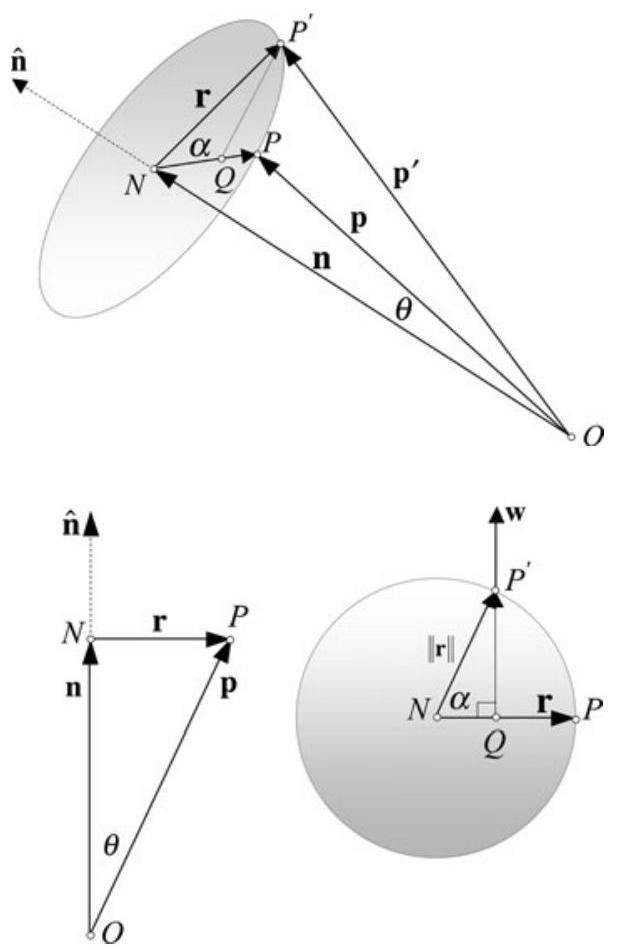
\includegraphics[max width=\textwidth, center]{2023_01_16_a848224efad29cd66460g-095}

where

$$
K=1-\cos \alpha .
$$

\subsection{向量}
Now let's solve the same problem using vectors. Figure $6.7$ shows a view of the geometry associated with the task at hand. For clarification, Fig. $6.8$ shows a crosssection and a plan view of the geometry.

The axis of rotation is given by the unit vector

$$
\hat{\mathbf{n}}=a \mathbf{i}+b \mathbf{j}+c \mathbf{k} .
$$

$P\left(x_{p}, y_{p} z_{p}\right)$ is the point to be rotated by angle $\alpha$ to $P^{\prime}\left(x_{p}^{\prime}, y_{p}^{\prime}, z_{p}^{\prime}\right)$.

$O$ is the origin, whilst $\mathbf{p}$ and $\mathbf{p}^{\prime}$ are position vectors for $P$ and $P^{\prime}$ respectively.

From Figs. $6.7$ and 6.8:

$$
\mathbf{p}^{\prime}=\overrightarrow{O N}+\overrightarrow{N Q}+\overrightarrow{Q P^{\prime}}
$$

To find $\overrightarrow{O N}$

$$
|\mathbf{n}|=|\mathbf{p}| \cos \theta=\hat{\mathbf{n}} \cdot \mathbf{p}
$$

therefore,

$$
\overrightarrow{O N}=\mathbf{n}=\hat{\mathbf{n}}(\hat{\mathbf{n}} \cdot \mathbf{p})
$$

To find $\overrightarrow{N Q}$ :

$$
\overrightarrow{N Q}=\frac{N Q}{N P} \mathbf{r}=\frac{N Q}{N P^{\prime}} \mathbf{r}=\cos \alpha \mathbf{r}
$$

but

$$
\mathbf{p}=\mathbf{n}+\mathbf{r}=\hat{\mathbf{n}}(\hat{\mathbf{n}} \cdot \mathbf{p})+\mathbf{r}
$$

therefore,

$$
\mathbf{r}=\mathbf{p}-\hat{\mathbf{n}}(\hat{\mathbf{n}} \cdot \mathbf{p})
$$

and

$$
\overrightarrow{N Q}=[\mathbf{p}-\hat{\mathbf{n}}(\hat{\mathbf{n}} \cdot \mathbf{p})] \cos \alpha
$$

To find $\overrightarrow{Q P^{\prime}}$ :

Let

$$
\hat{\mathbf{n}} \times \mathbf{p}=\mathbf{w}
$$

where

$$
|\mathbf{w}|=|\hat{\mathbf{n}}| \cdot|\mathbf{p}| \sin \theta=|\mathbf{p}| \sin \theta
$$

but

$$
|\mathbf{r}|=|\mathbf{p}| \sin \theta
$$

therefore,

$$
|\mathbf{w}|=|\mathbf{r}| .
$$

Now

$$
\frac{Q P^{\prime}}{N P^{\prime}}=\frac{Q P^{\prime}}{|\mathbf{r}|}=\frac{Q P^{\prime}}{|\mathbf{w}|}=\sin \alpha
$$

therefore,

$$
\overrightarrow{Q P^{\prime}}=\mathbf{w} \sin \alpha=(\hat{\mathbf{n}} \times \mathbf{p}) \sin \alpha
$$

then

$$
\mathbf{p}^{\prime}=\hat{\mathbf{n}}(\hat{\mathbf{n}} \cdot \mathbf{p})+(\mathbf{p}-\hat{\mathbf{n}}(\hat{\mathbf{n}} \cdot \mathbf{p})) \cos \alpha+(\hat{\mathbf{n}} \times \mathbf{p}) \sin \alpha
$$

and

$$
\mathbf{p}^{\prime}=\mathbf{p} \cos \alpha+\hat{\mathbf{n}}(\hat{\mathbf{n}} \cdot \mathbf{p})(1-\cos \alpha)+(\hat{\mathbf{n}} \times \mathbf{p}) \sin \alpha .
$$

Let

$$
K=1-\cos \alpha
$$

Fig. 6.9 Rotating the point $P$ through $180^{\circ}$ to $P^{\prime}$

\begin{center}
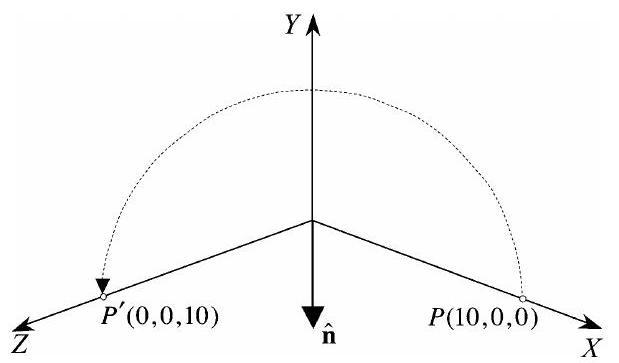
\includegraphics[max width=\textwidth]{2023_01_16_a848224efad29cd66460g-097}
\end{center}

then

$$
\mathbf{p}^{\prime}=\mathbf{p} \cos \alpha+\hat{\mathbf{n}}(\hat{\mathbf{n}} \cdot \mathbf{p}) K+(\hat{\mathbf{n}} \times \mathbf{p}) \sin \alpha
$$

and

$$
\begin{aligned}
\mathbf{p}^{\prime}= & \left(x_{p} \mathbf{i}+y_{p} \mathbf{j}+z_{p} \mathbf{k}\right) \cos \alpha+(a \mathbf{i}+b \mathbf{j}+c \mathbf{k})\left(a x_{p}+b y_{p}+c z_{p}\right) K \\
& +\left[\left(b z_{p}-c y_{p}\right) \mathbf{i}+\left(c x_{p}-a z_{p}\right) \mathbf{j}+\left(a y_{p}-b x_{p}\right) \mathbf{k}\right] \sin \alpha \\
\mathbf{p}^{\prime}= & {\left[x_{p} \cos \alpha+a\left(a x_{p}+b y_{p}+c z_{p}\right) K+\left(b z_{p}-c y_{p}\right) \sin \alpha\right] \mathbf{i} } \\
& +\left[y_{p} \cos \alpha+b\left(a x_{p}+b y_{p}+c z_{p}\right) K+\left(c x_{p}-a z_{p}\right) \sin \alpha\right] \mathbf{j} \\
& +\left[z_{p} \cos \alpha+c\left(a x_{p}+b y_{p}+c z_{p}\right) K+\left(a y_{p}-b x_{p}\right) \sin \alpha\right] \mathbf{k} \\
\mathbf{p}^{\prime}= & {\left[x_{p}\left(a^{2} K+\cos \alpha\right)+y_{p}(a b K-c \sin \alpha)+z_{p}(a c K+b \sin \alpha)\right] \mathbf{i} } \\
& +\left[x_{p}(a b K+c \sin \alpha)+y_{p}\left(b^{2} K+\cos \alpha\right)+z_{p}(b c K-a \sin \alpha)\right] \mathbf{j} \\
& +\left[x_{p}(a c K-b \sin \alpha)+y_{p}(b c K+a \sin \alpha)+z_{p}\left(c^{2} K+\cos \alpha\right)\right] \mathbf{k}
\end{aligned}
$$

which unpacks into the transform:

$$
\left[\begin{array}{c}
x_{p}^{\prime} \\
y_{p}^{\prime} \\
z_{p}^{\prime}
\end{array}\right]=\left[\begin{array}{ccc}
a^{2} K+\cos \alpha & a b K-c \sin \alpha & a c K+b \sin \alpha \\
a b K+c \sin \alpha & b^{2} K+\cos \alpha & b c K-a \sin \alpha \\
a c K-b \sin \alpha & b c K+a \sin \alpha & c^{2} K+\cos \alpha
\end{array}\right]\left[\begin{array}{c}
x_{p} \\
y_{p} \\
z_{p}
\end{array}\right]
$$

where

$$
K=1-\cos \alpha
$$

and is identical to the transform derived using matrices.

Let's test the transform with a simple example that can be easily verified. If we rotate the point $P(10,0,0), 180^{\circ}$ about an axis defined by $\hat{\mathbf{n}}=(1 / \sqrt{2}) \mathbf{i}+(1 / \sqrt{2}) \mathbf{k}$, it should be rotated to $P^{\prime}(0,0,10)$ as shown in Fig. 6.9. Therefore,

$$
\begin{gathered}
\alpha=180^{\circ}, \quad \cos \alpha=-1, \quad \sin \alpha=0, \quad K=2, \\
a=\frac{1}{\sqrt{2}}, \quad b=0, \quad c=\frac{1}{\sqrt{2}}
\end{gathered}
$$

and

$$
\left[\begin{array}{c}
0 \\
0 \\
10
\end{array}\right]=\left[\begin{array}{ccc}
0 & 0 & 1 \\
0 & -1 & 0 \\
1 & 0 & 0
\end{array}\right]\left[\begin{array}{c}
10 \\
0 \\
0
\end{array}\right]
$$

which confirms our prediction.

\section{总结}
In this chapter we have reviewed the matrix rotation transforms for rotating a point about one of the three Cartesian axes. By employing homogeneous coordinates, the translation transform can be integrated to rotate points about an off-set axis parallel with one of the Cartesian axes.

Composite rotations are created by combining the matrices representing the individual rotations about three successive axes. Such rotations are known as Euler rotations, and there are twelve ways of combining these matrices. Unfortunately, one of the problems with such transforms is that they suffer from gimbal lock, where one degree of freedom is lost under certain angle combinations. Another problem, is that it is difficult to predict how a point moves in space when animated by a composite transform, although they are widely used for positioning objects in world space.

Finally, matrices and vectors were used to develop a transform for rotating a point about an arbitrary axis.

\subsection{变换总结}
\subsubsection*{Translate a point}
$$
\mathbf{T}_{t_{x}, t_{y}, t_{z}}=\left[\begin{array}{cccc}
1 & 0 & 0 & t_{x} \\
0 & 1 & 0 & t_{y} \\
0 & 0 & 1 & t_{z} \\
0 & 0 & 0 & 1
\end{array}\right]
$$

\subsubsection*{Rotate a point about the $x-, y-, z$-axes}
$$
\begin{aligned}
\mathbf{R}_{\beta, x}= & {\left[\begin{array}{ccc}
1 & 0 & 0 \\
0 & \cos \beta & -\sin \beta \\
0 & \sin \beta & \cos \beta
\end{array}\right] } \\
\mathbf{R}_{\beta, y}= & {\left[\begin{array}{ccc}
\cos \beta & 0 & \sin \beta \\
0 & 1 & 0 \\
-\sin \beta & 0 & \cos \beta
\end{array}\right] } \\
\mathbf{R}_{\beta, z}= & {\left[\begin{array}{ccc}
\cos \beta & -\sin \beta & 0 \\
\sin \beta & \cos \beta & 0 \\
0 & 0 & 1
\end{array}\right] }
\end{aligned}
$$

\subsubsection*{Rotate a point about off-set $x-, y-, z$-axes}
$$
\begin{aligned}
\mathbf{R}_{\beta, x,\left(0, t_{y}, t_{z}\right)} & =\left[\begin{array}{cccc}
1 & 0 & 0 & 0 \\
0 & \cos \beta & -\sin \beta & t_{y}(1-\cos \beta)+t_{z} \sin \beta \\
0 & \sin \beta & \cos \beta & t_{z}(1-\cos \beta)-t_{y} \sin \beta \\
0 & 0 & 0 & 1
\end{array}\right] \\
\mathbf{R}_{\beta, y,\left(t_{x}, 0, t_{z}\right)} & =\left[\begin{array}{cccc}
\cos \beta & 0 & \sin \beta & t_{x}(1-\cos \beta)-t_{z} \sin \beta \\
0 & 1 & 0 & 0 \\
-\sin \beta & 0 & \cos \beta & t_{z}(1-\cos \beta)+t_{x} \sin \beta \\
0 & 0 & 0 & 1
\end{array}\right] \\
\mathbf{R}_{\beta, z,\left(t_{x}, t_{y}, 0\right)} & =\left[\begin{array}{cccc}
\cos \beta & -\sin \beta & 0 & t_{x}(1-\cos \beta)+t_{y} \sin \beta \\
\sin \beta & \cos \beta & 0 & t_{y}(1-\cos \beta)-t_{x} \sin \beta \\
0 & 0 & 1 & 0 \\
0 & 0 & 0 & 1
\end{array}\right]
\end{aligned}
$$

\subsubsection*{Rotate a point about an arbitrary axis}
$$
\begin{aligned}
\mathbf{R}_{\alpha, \hat{\mathbf{n}}} & =\left[\begin{array}{ccc}
a^{2} K+\cos \alpha & a b K-c \sin \alpha & a c K+b \sin \alpha \\
a b K+c \sin \alpha & b^{2} K+\cos \alpha & b c K-a \sin \alpha \\
a c K-b \sin \alpha & b c K+a \sin \alpha & c^{2} K+\cos \alpha
\end{array}\right] \\
K & =1-\cos \alpha \\
\hat{\mathbf{n}} & =a \mathbf{i}+b \mathbf{j}+c \mathbf{k} .
\end{aligned}
$$

\section{样例}
Here are some further worked examples that employ the ideas described above. In some cases, a test is included to confirm the result.

Example 1 Develop a rotation transform to rotate a point about an axis off-set to the $y$-axis.

Let the off-set axis intersect the point $\left(t_{x}, 0, t_{z}\right)$. Therefore, the homogeneous transform for this rotation is

$$
\left[\begin{array}{c}
x^{\prime} \\
y^{\prime} \\
z^{\prime} \\
1
\end{array}\right]=\mathbf{T}_{t_{x}, 0, t_{z}} \mathbf{R}_{\beta, y} \mathbf{T}_{-t_{x}, 0,-t_{z}}\left[\begin{array}{c}
x \\
y \\
z \\
1
\end{array}\right]
$$

where

$$
\begin{aligned}
& \mathbf{T}_{-t_{x}, 0,-t_{z}} \quad \text { creates a temporary origin } \\
& \mathbf{R}_{\beta, y} \quad \text { rotates } \beta \text { about the temporary } y \text {-axis } \\
& \mathbf{T}_{t_{x}, 0, t_{z}} \quad \text { returns to the original position }
\end{aligned}
$$

and

$$
\begin{aligned}
\mathbf{T}_{t_{x}, 0, t_{z}} & =\left[\begin{array}{llll}
1 & 0 & 0 & t_{x} \\
0 & 1 & 0 & 0 \\
0 & 0 & 1 & t_{z} \\
0 & 0 & 0 & 1
\end{array}\right] \\
\mathbf{T}_{-t_{x}, 0,-t_{z}} & =\left[\begin{array}{cccc}
1 & 0 & 0 & -t_{x} \\
0 & 1 & 0 & 0 \\
0 & 0 & 1 & -t_{z} \\
0 & 0 & 0 & 1
\end{array}\right] \\
\mathbf{R}_{\beta, y} & =\left[\begin{array}{cccc}
\cos \beta & 0 & \sin \beta & 0 \\
0 & 1 & 0 & 0 \\
-\sin \beta & 0 & \cos \beta & 0 \\
0 & 0 & 0 & 1
\end{array}\right] .
\end{aligned}
$$

Therefore,

$$
\begin{aligned}
& \mathbf{T}_{t_{x}, 0, t_{z}} \mathbf{R}_{\beta, y} \mathbf{T}_{-t_{x}, 0,-t_{z}} \\
&= {\left[\begin{array}{cccc}
1 & 0 & 0 & t_{x} \\
0 & 1 & 0 & 0 \\
0 & 0 & 1 & t_{z} \\
0 & 0 & 0 & 1
\end{array}\right]\left[\begin{array}{cccc}
\cos \beta & 0 & \sin \beta & 0 \\
0 & 1 & 0 & 0 \\
-\sin \beta & 0 & \cos \beta & 0 \\
0 & 0 & 0 & 1
\end{array}\right]\left[\begin{array}{cccc}
1 & 0 & 0 & -t_{x} \\
0 & 1 & 0 & 0 \\
0 & 0 & 1 & -t_{z} \\
0 & 0 & 0 & 1
\end{array}\right] } \\
&= {\left[\begin{array}{cccc}
1 & 0 & 0 & t_{x} \\
0 & 1 & 0 & 0 \\
0 & 0 & 1 & t_{z} \\
0 & 0 & 0 & 1
\end{array}\right]\left[\begin{array}{cccc}
\cos \beta & 0 & \sin \beta & -t_{x} \cos \beta-t_{z} \sin \beta \\
0 & 1 & 0 & 0 \\
-\sin \beta & 0 & \cos \beta & t_{x} \sin \beta-t_{z} \cos \beta \\
0 & 0 & 0 & 1
\end{array}\right] } \\
&= {\left[\begin{array}{ccccc}
\cos \beta & 0 & \sin \beta & t_{x}(1-\cos \beta)-t_{z} \sin \beta \\
0 & 1 & 0 & 0 \\
-\sin \beta & 0 & \cos \beta & t_{z}(1-\cos \beta)+t_{x} \sin \beta \\
0 & 0 & 0 & 1
\end{array}\right] }
\end{aligned}
$$

Example 2 Compute the rotation transform for $\mathbf{R}_{\gamma, x} \mathbf{R}_{\beta, y} \mathbf{R}_{\alpha, x}$ and see if it suffers from gimbal lock when $\alpha=\beta=\gamma=90^{\circ}$. What is the axis and angle of rotation?

Using the notation $c_{\beta}=\cos \beta$ and $s_{\beta}=\sin \beta$, the composite transform is

$$
\begin{aligned}
\mathbf{R}_{\gamma, x} \mathbf{R}_{\beta, y} \mathbf{R}_{\alpha, x} & =\left[\begin{array}{ccc}
1 & 0 & 0 \\
0 & c_{\gamma} & -s_{\gamma} \\
0 & s_{\gamma} & c_{\gamma}
\end{array}\right]\left[\begin{array}{ccc}
c_{\beta} & 0 & s_{\beta} \\
0 & 1 & 0 \\
-s_{\beta} & 0 & c_{\beta}
\end{array}\right]\left[\begin{array}{ccc}
1 & 0 & 0 \\
0 & c_{\alpha} & -s_{\alpha} \\
0 & s_{\alpha} & c_{\alpha}
\end{array}\right] \\
& =\left[\begin{array}{ccc}
c_{\beta} & s_{\beta} s_{\alpha} & s_{\beta} c_{\alpha} \\
s_{\gamma} s_{\beta} & \left(c_{\gamma} c_{\alpha}-s_{\gamma} c_{\beta} s_{\alpha}\right) & \left(-c_{\gamma} s_{\alpha}-s_{\gamma} c_{\beta} c_{\alpha}\right) \\
-c_{\gamma} s_{\beta} & \left(s_{\gamma} c_{\alpha}+c_{\gamma} c_{\beta} s_{\alpha}\right) & \left(-s_{\gamma} s_{\alpha}+c_{\gamma} c_{\beta} c_{\alpha}\right)
\end{array}\right] \\
\mathbf{R}_{90^{\circ}, x} \mathbf{R}_{90^{\circ}, y} \mathbf{R}_{90^{\circ}, x} & =\left[\begin{array}{ccc}
0 & 1 & 0 \\
1 & 0 & 0 \\
0 & 0 & -1
\end{array}\right] .
\end{aligned}
$$

Figure $6.10$ shows a cube at each stage of rotation, and it is clear that gimbal lock is not present as the cube is rotated through each of its orthogonal axes. The axis (a)

\begin{center}
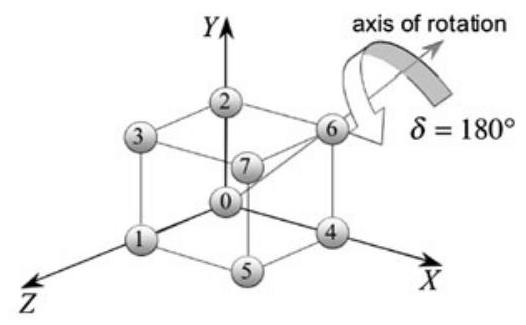
\includegraphics[max width=\textwidth]{2023_01_16_a848224efad29cd66460g-101}
\end{center}

(c)

\begin{center}
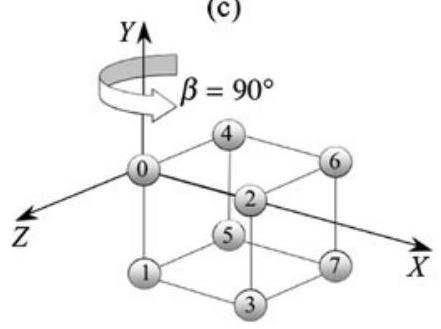
\includegraphics[max width=\textwidth]{2023_01_16_a848224efad29cd66460g-101(1)}
\end{center}

(b)

\begin{center}
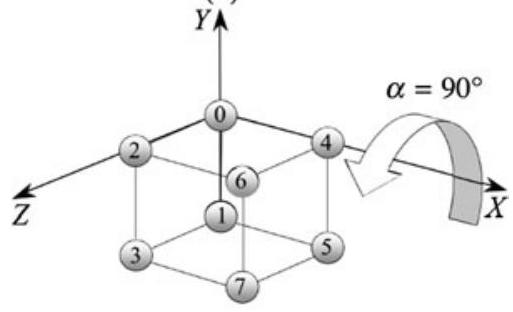
\includegraphics[max width=\textwidth]{2023_01_16_a848224efad29cd66460g-101(2)}
\end{center}

(d)

\begin{center}
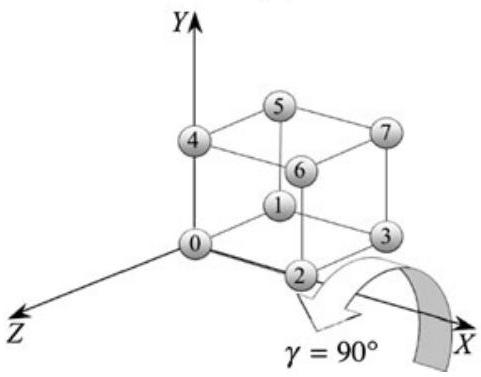
\includegraphics[max width=\textwidth]{2023_01_16_a848224efad29cd66460g-101(3)}
\end{center}

Fig. 6.10 Four views of the unit cube before and during the three rotations $\mathbf{R}_{90^{\circ}, x} \mathbf{R}_{90^{\circ}, y} \mathbf{R}_{90^{\circ}, x}$

of rotation is through the vertices 0 and 6, i.e. $\left[\begin{array}{lll}1 & 1 & 0\end{array}\right]^{\mathrm{T}}$ and the angle of rotation is $180^{\circ}$.

Example 3 Show that the rotation matrix for rotating points about an arbitrary axis works for the three Cartesian axes.

Starting with the matrix:

$$
\begin{aligned}
\mathbf{R}_{\alpha, \hat{\mathbf{n}}} & =\left[\begin{array}{ccc}
a^{2} K+\cos \alpha & a b K-c \sin \alpha & a c K+b \sin \alpha \\
a b K+c \sin \alpha & b^{2} K+\cos \alpha & b c K-a \sin \alpha \\
a c K-b \sin \alpha & b c K+a \sin \alpha & c^{2} K+\cos \alpha
\end{array}\right] \\
K & =1-\cos \alpha \\
\hat{\mathbf{n}} & =a \mathbf{i}+b \mathbf{j}+c \mathbf{k} .
\end{aligned}
$$

Rotating about the $x$-axis:

$$
\hat{\mathbf{n}}=a \mathbf{i}
$$

therefore, $a=1$ and $b=c=0$ :

$$
\mathbf{R}_{\alpha, x}=\left[\begin{array}{ccc}
1 & 0 & 0 \\
0 & \cos \alpha & -\sin \alpha \\
0 & \sin \alpha & \cos \alpha
\end{array}\right] .
$$

Rotating about the $y$-axis:

$$
\hat{\mathbf{n}}=b \mathbf{j}
$$

therefore, $b=1$ and $a=c=0$ :

$$
\mathbf{R}_{\alpha, y}=\left[\begin{array}{ccc}
\cos \alpha & 0 & \sin \alpha \\
0 & 1 & 0 \\
-\sin \alpha & 0 & \cos \alpha
\end{array}\right]
$$

Rotating about the $z$-axis:

$$
\hat{\mathbf{n}}=c \mathbf{k}
$$

therefore, $c=1$ and $a=b=0$ :

$$
\mathbf{R}_{\alpha, z}=\left[\begin{array}{ccc}
\cos \alpha & -\sin \alpha & 0 \\
\sin \alpha & \cos \alpha & 0 \\
0 & 0 & 1
\end{array}\right]
$$

which are correct.

Example 4 Compute the rotation transform to rotate a point $180^{\circ}$ about an axis aligned with $\left[\begin{array}{lll}1 & 1 & 1\end{array}\right]^{\mathrm{T}}$. Show by example, that rotating a point twice by this transform returns it to its original position.

Starting with the matrix:

$$
\begin{aligned}
\mathbf{R}_{\alpha, \hat{\mathbf{n}}} & =\left[\begin{array}{ccc}
a^{2} K+\cos \alpha & a b K-c \sin \alpha & a c K+b \sin \alpha \\
a b K+c \sin \alpha & b^{2} K+\cos \alpha & b c K-a \sin \alpha \\
a c K-b \sin \alpha & b c K+a \sin \alpha & c^{2} K+\cos \alpha
\end{array}\right] \\
K & =1-\cos \alpha \\
\hat{\mathbf{n}} & =a \mathbf{i}+b \mathbf{j}+c \mathbf{k} .
\end{aligned}
$$

Therefore, given $\mathbf{n}=\mathbf{i}+\mathbf{j}+\mathbf{k}$

$$
\hat{\mathbf{n}}=\frac{1}{\sqrt{3}} \mathbf{i}+\frac{1}{\sqrt{3}} \mathbf{j}+\frac{1}{\sqrt{3}} \mathbf{k}
$$

and

$$
a=b=c=\frac{1}{\sqrt{3}} \text {. }
$$

Given $\alpha=180^{\circ}, \cos \alpha=-1, \sin \alpha=0$ and $K=2$, and the matrix becomes:

$$
\mathbf{R}_{180^{\circ}, \hat{\mathbf{n}}}=\left[\begin{array}{ccc}
-1 / 3 & 2 / 3 & 2 / 3 \\
2 / 3 & -1 / 3 & 2 / 3 \\
2 / 3 & 2 / 3 & -1 / 3
\end{array}\right] \text {. }
$$

Multiplying this matrix by itself must result in the identity matrix:

$$
\begin{aligned}
\mathbf{R}_{180^{\circ}, \hat{\mathbf{n}}} \mathbf{R}_{180^{\circ}, \hat{\mathbf{n}}} & =\left[\begin{array}{ccc}
-1 / 3 & 2 / 3 & 2 / 3 \\
2 / 3 & -1 / 3 & 2 / 3 \\
2 / 3 & 2 / 3 & -1 / 3
\end{array}\right]\left[\begin{array}{ccc}
-1 / 3 & 2 / 3 & 2 / 3 \\
2 / 3 & -1 / 3 & 2 / 3 \\
2 / 3 & 2 / 3 & -1 / 3
\end{array}\right] \\
& =\left[\begin{array}{ccc}
1 & 0 & 0 \\
0 & 1 & 0 \\
0 & 0 & 1
\end{array}\right]
\end{aligned}
$$

which confirms that any point rotated twice by the rotation matrix returns to its original point.
